\graphicspath{{content/2_design/figures/}}
\section{Serial Communication}

A serial communication protocol and procedure will be implemented that will allow control of the car, as well as telemetry readings.
The protocol will be implemented over UART and Bluetooth to allow both USB and wireless control. The protocol will set out
the rules for communication between a "client" and a "server". This will define the types of messages and the format of the data.
The protocol will then be implemented by the server (ESP) and the client (PC) respectively.

\subsection{Protocol}

Table \ref{tab:protocolMessages} shows the list of messages that may either be sent by the client (a "request"),
or sent by the server (a "response"). Each message consists of an ID followed by a potential payload.
IDs 000 to 099 are reserved for "get" messages, and 100 to 199 are reserved for "set" messages.
\textit{Payload} refers to the data that will be sent be either the client \textit{or} the server.
\textit{void} implies that either the client \textit{or} the server must NOT pass any payload for that message.
\textit{N/A} implies that either the client \textit{or} the server must NEVER send that message.

\begin{table}[!htb]
  \centering
  \renewcommand{\arraystretch}{1.2}
  \begin{tabular}{ |c|c|c|c| }
    \hline
    \textbf{Description}         & \textbf{ID}        & \textbf{Payload (from client)}      & \textbf{Payload (from server)}    \\
    \hline
    Get All Information          & [000]              & void                                & [ID][Payload] for each "get"      \\
    \hline
    Get Left Wheel Current       & [001]              & void                                & [float32] (mA)                    \\
    \hline
    Get Right Wheel Current      & [002]              & void                                & [float32] (mA)                    \\
    \hline
    Get Left Sensor Range        & [003]              & void                                & [float32] (mm)                    \\
    \hline
    Get Right Sensor Range       & [004]              & void                                & [float32] (mm)                    \\
    \hline
    Get Battery Voltage          & [005]              & void                                & [float32] (mV)                    \\
    \hline
    Get Left Wheel Speed         & [006]              & void                                & [uint8]                           \\
    \hline
    Get Right Wheel Speed        & [007]              & void                                & [uint8]                           \\
    \hline
    Set Left Wheel Speed         & [100]              & [uint8]                             & N/A                               \\
    \hline
    Set Right Wheel Speed        & [101]              & [uint8]                             & N/A                               \\
    \hline
  \end{tabular}
  \caption{}
  \label{tab:protocolMessages}
\end{table}

\subsection{ESP Firmware}

The firmware on the ESP should be designed to be both scalable yet fast. The setup for the protocol is trivial - UART is already
initialized in the Arduino framework, and bluetooth simply needs to be initialized with a single function call.

The flow diagram in Figure \ref{fig:serialCommunication_firmwareDiagram} therefore illustrates the implementation of the protocol
in the main loop. Note that because the length of the message is known, there is no need for a state machine - the firmware
can simply wait on the serial buffer until it is populated to the required length for that message.

\begin{figure}[!htb]
  \centering
  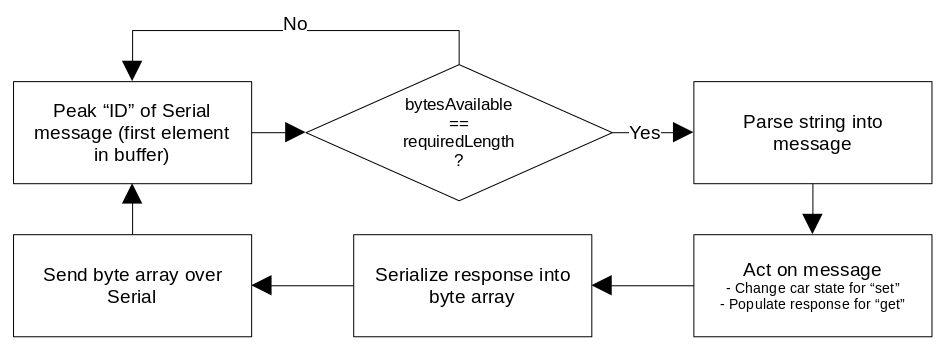
\includegraphics[width=0.9\textwidth]{serialCommunication_firmwareDiagram}
  \caption{Serial Communication Firmware Flow Diagram}
  \label{fig:serialCommunication_firmwareDiagram}
\end{figure}

\subsection{PC Software}

The software from the PC should provided a command-line interface to command the car's wheel speeds and to get telemetry readings.
The implementation is relatively simple:

\begin{enumerate}
  \item Start a connection with the device via either serial or bluetooth when the application starts.
  \item Wait for any "commands" from the user e.g. "set lws 8" to set the left wheel speed to 8 while the application is running.
  \item Parse the arguments of the user's command into a Message structure.
  \item Serialize the Message into a byte array.
  \item Send the byte array over the relevant protocol.
  \item If the Message is a "get" request, block and wait for a response for a short amount of time:
  \begin{enumerate}
    \item Receive the Message response over the relevant protocol.
    \item Deserialize the byte array into a Message structure.
    \item Display the results of the Message to the user.
  \end{enumerate}
\end{enumerate}